\chapter{Methodology}
\label{chap:met}

This chapter will present a detailed explanation of the principles underlying the 
proposed methodology. The section \ref{sec:rigid_body_and_const} offers a concise 
overview of rigid-body systems and constraints that can be imposed on them.
The next section \ref{sec:udwadia_kalaba_app} introduces the Udwadia-Kalaba 
approach and physical principles that stays behind it. Further in Section 
\ref{sec:def_rigid_body_const}, this technique is applied to solve the discussed 
problem. Then Section \ref{sec:control_through_udwadia} use the Udwadia-Kalaba 
approach to construct a control law. Finally, Section 
\ref{sec:task_prioritization} contains thoughts about prioritization constraint 
task over control one. 

\section{Rigid-body systems and constraints} 
\label{sec:rigid_body_and_const}

The most common class of physical systems that can be observed in the real life 
cases is the rigid-body one. Some examples of such systems are demonstrated in 
Figure \ref{fig:examples_of_rig_sys}. The key feature of rigid-body systems 
is non-deformable parts that forms it. With these limitations only an 
inner stiffness can be described.

\begin{figure}[H]
    \centering
    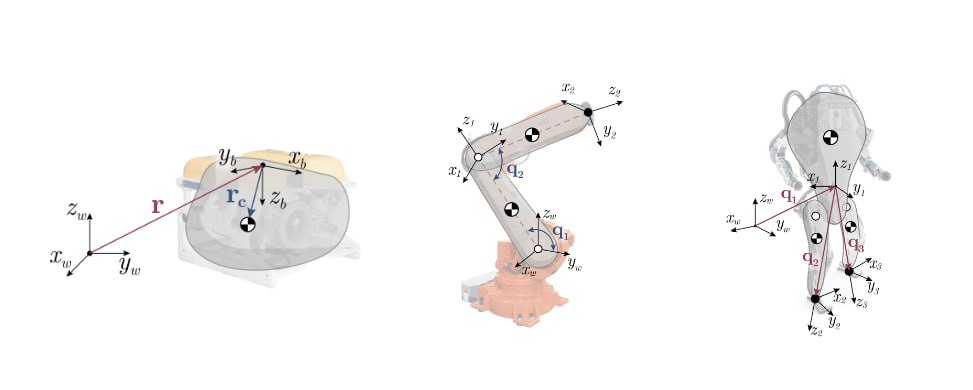
\includegraphics[scale=0.5]{figs/rigid_body_systems.png}
    \caption{Examples of rigid-body systems}
    \label{fig:examples_of_rig_sys}
\end{figure}


Nevertheless, the mathematical tools to work with rigid-body systems was introduced 
in \RNum{18}-th century by Newton and Euler works. Using this approach it is easy 
to formulate a set f deferential equations that describes the system behavior.
However, in this study the another (more convenient) technique is utilized. It is 
called the least action principle. The formulation is the following equation

\begin{equation}
    \min_{\mathbf{q}} \quad 
    \int_{t_1}^{t_2} L(\mathbf{q}(t), \mathbf{v}(t), t) dt
    \label{eqn:least_act_principle}
\end{equation}

where $L$ is Lagrangian of the system, and $\mathbf{q}$, $\mathbf{v}$ are 
functions of the generalized coordinates and velocities respectively. The solution 
of the variational problem (\ref{eqn:least_act_principle}) is the Euler-Lagrange 
differential equations. The solution through utilizing the Lagrangian can be 
easily generalized to all rigid-body systems. This generalization is aforementioned 
the canonical manipulator equation (\ref{eqn:can_man_equation}). 

In this chapter the convenient representation of this equation is used. The main 
idea of rewriting is combination of the inertial forces with non-inertial ones.

\begin{equation}
    M \dot{\mathbf{v}} = \mathbf{Q}
    \label{eqn:can_man_eqn_simple}
\end{equation}

In the above equation $\mathbf{Q} = 
-C(\mathbf{q}, \mathbf{v}) \dot{\mathbf{q}} - g(\mathbf{q}) + 
\boldsymbol{\tau}$, $M \succcurlyeq 0$ is inertia matrix, $C$ is Centrifugal-Coriolis 
matrix, $g$ is gradient of conservative forces. The dependency from coordinates and 
velocities is amended for convenience. In the most generalized case 
$\dim{\mathbf{q}} = n_q \neq n_v = \dim{\mathbf{v}}$.

The aforementioned description is applicable for open and closed loop systems. 
The closed one is described in Figure \ref{fig:rigid_coupling}. However, 
as mentioned above utilizing only equation \ref{eqn:can_man_eqn_simple} to handle 
such system is not efficient. Thus, the approach via constraints described
by equation (\ref{eqn:holonom_const}) is more preferable. It can be inserted in 
(\ref{eqn:least_act_principle}), which leads to the following variational problem, 

\begin{equation}
    \min_{\mathbf{q}} \quad 
    \int_{t_1}^{t_2} [L(\mathbf{q}(t), \mathbf{v}(t), t) - 
    \pmb{\lambda}^T \varphi(\mathbf{q}(t), t)]dt
    \label{eqn:least_act_principle_const}
\end{equation}

The solution the above equation can be expressed in terms of the KKT matrix in 
the following way, 

\begin{equation}
    \begin{bmatrix}
        M & J^T \\
        J & 0 \\
    \end{bmatrix}
    \begin{bmatrix}
        \dot{\mathbf{v}} \\
        -\pmb{\lambda}
    \end{bmatrix} = 
    \begin{bmatrix}
        \mathbf{Q} \\
        -\dot{J} \mathbf{v}
    \end{bmatrix}, \:
    J = \frac{\partial \boldsymbol{\varphi}}{\partial \mathbf{q}}
    \label{eqn:kkt_solution}
\end{equation}

The downside of the equation (\ref{eqn:kkt_solution}) is that it does not support 
non-holonomic constraints generally. This type of constraints can be defined as 

\begin{equation}
    \varphi(\mathbf{q}, \mathbf{v}, t) = 0
    \label{eqn:non_holonomic_const}
\end{equation}

Therefore, the dependency from generalized velocity makes the KKT approach not 
applicable. The handle of such constraints is crucial for defining a control. 
Hence, it is necessary to use another technique.

\section{The Udwadia-Kalaba approach} \label{sec:udwadia_kalaba_app}

The main differences of the Udwadia-Kalaba approach from the method mentioned 
above are the another view on constraints, and utilizing different physical 
principle.

Let's start from reviewing the constraints form in the discussed technique. It 
can be derived from holonomic and non-holonomic type by differentiating over time, 
and transforming to an affine form. The general equation is the following 

\begin{equation}
    A(\mathbf{q}, \mathbf{v}, t) \dot{\mathbf{v}} = 
    \mathbf{b}(\mathbf{q}, \mathbf{v}, t)
    \label{eqn:affine_const}
\end{equation}

The above equation can be used in the Gauss least constraint principle. For further 
convenience the arguments of matrix functions is amended. It leads to the 
following optimization problem:

\begin{equation}
    \begin{aligned}
        \min_{\dot{\mathbf{v}}} \quad &
        [\dot{\mathbf{v}} - \mathbf{a}]^T M [\dot{\mathbf{v}} - \mathbf{a}] \\
        \textrm{s.t.} \quad &
        A \dot{\mathbf{v}} = \mathbf{b} \\
        &
        \mathbf{a} = M^{-1} \mathbf{Q}
    \end{aligned}
    \label{eqn:gauss_least_const}
\end{equation}

This optimization can be solved analytically as Ferdaus Udwadia and Robert Kalaba 
demonstrated \cite{UdwadiaKalabaApproach}. This solution is shown below.

\begin{equation}
    \dot{\mathbf{v}} = 
    \mathbf{a} + M^{-1 / 2}(A M^{-1 / 2})^+ (\mathbf{b} - AM^{-1} \mathbf{Q})
    \label{eqn:udwadia_kalaba_sol}
\end{equation}

where $[\cdot]^+$ is the Moore-Penrose inverse, and 
$M^{\pm 1 / 2} = W \Lambda^{\pm 1 / 2} W^T$, $W$ is the orthogonal matrix 
of eigen vectors. 

In case of positive semi-definiteness of $M$ the equation 
(\ref{eqn:udwadia_kalaba_sol}) is not applicable because $M^{-1}$, 
$M^{-1 / 2}$ cannot exist. The Firdaus Udwadia and Aaron Schutte demonstrates 
\cite{EquationsOfMotionConst} a methodology to bypass this problem by 
replacing $M$, and $\mathbf{a}$ by the following quantities respectively

\begin{equation}
    \begin{aligned}
        M_A = M + A^+ A \succ 0 \\
        \mathbf{a}_A = M_A^{-1} \mathbf{Q}
    \end{aligned}
    \label{eqn:another_mass_matrix}
\end{equation}

Utilizing the mentioned quantities it is possible to define constraints 
force over the wide range of rigid-body systems. These forces can be 
expressed in the following manner 

\begin{equation}
    \mathbf{Q}_C = M^{1 / 2} (A M^{-1 /2})^+(\mathbf{b} - AM^{-1} \mathbf{Q})
    \label{eqn:constraint_forces}
\end{equation}

Hence, the Udwadia-Kalaba approach is applicable for emulation a of 
rigid body constraint in computation easily. Only the problem with rigorous 
defining $A$ and $\mathbf{b}$ remains.

\section{Defying rigid body constraint}
\label{sec:def_rigid_body_const}

As mentioned above the discussed coupling between physical systems is created 
by some rigid body. This type of mathematical object can be described by the 
following identity for any two points

\begin{equation}
    \| \mathbf{r}_A(t) - \mathbf{r}_B(t) \| \equiv \text{const}
    \label{eqn:rigid_body_axiom}
\end{equation}

From the above equation kinematic laws can be directly derived. For further 
investigations it is necessary to introduce a point velocity of the rigid body

\begin{figure}[H]
    \centering
    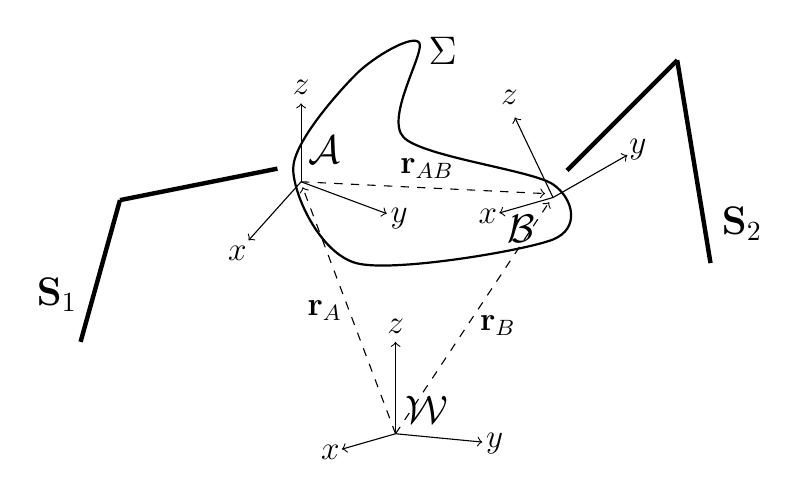
\begin{tikzpicture}[
        media/.style={font={\footnotesize\sffamily}},
        interface/.style={
            % The border decoration is a path replacing decorator.
            % For the interface style we want to draw the original path.
            % The postaction option is therefore used to ensure that the
            % border decoration is drawn *after* the original path.
            postaction={draw,decorate,decoration={border,angle=-45,
            amplitude=0.3cm,segment length=2mm}}},
        ]
        % Object
        \draw [black, thick] plot [smooth cycle] coordinates {
            (2.7, 2.2) (3.5, 3.4) (4.3, 3.8) (4.1, 2.6) (6.0, 2.0) (6.0, 1.3) (3.5, 1.0)
        };
        \draw[media] (4.6, 3.7) node {\Large $\boldsymbol \Sigma$};

        % p_A
        \draw[black, ->, dashed](4.000, -1.167) -- (2.800 + 0.02, 2.033 - 0.07);
        \draw[media] (3.1, 0.40) node {\large $\mathbf{r}_A$}; 
        % p_B
        \draw[black, ->, dashed](4.000, -1.167) -- (6.000 - 0.05, 1.833 - 0.06);
        \draw[media] (5.3, 0.2) node {\large $\mathbf{r}_B$}; 
        % p_AB
        \draw[black, ->, dashed](2.800, 2.033) -- (6.000 - 0.1, 1.833 + 0.05);
        \draw[media] (4.4, 2.2) node {\large $\mathbf{r}_{AB}$};

        % world frame
        \draw[black, ->](4.000, -1.167) -- (5.102, -1.273);
        \draw[black, ->](4.000, -1.167) -- (4.000, 0.000);
        \draw[black, ->](4.000, -1.167) -- (3.318, -1.363);
        \drawdot{4.000}{-1.167}
        \draw[media] (4.400, -0.867) node {\Large $\mathcal{W}$}; 
        \draw[media] (5.260, -1.288) node {\large $y$}; 
        \draw[media] (4.000, 0.200) node {\large $z$}; 
        \draw[media] (3.172, -1.406) node {\large $x$}; 

        % A frame
        \draw[black, ->](2.800, 2.033) -- (3.889, 1.628);
        \draw[black, ->](2.800, 2.033) -- (2.800, 3.029);
        \draw[black, ->](2.800, 2.033) -- (2.133, 1.289);
        \drawdot{2.800}{2.033}
        \draw[media] (3.100, 2.433) node {\Large $\mathcal{A}$}; 
        \draw[media] (4.045, 1.570) node {\large $y$}; 
        \draw[media] (2.800, 3.230) node {\large $z$}; 
        \draw[media] (1.990, 1.130) node {\large $x$}; 

        % B frame
        \draw[black, ->](6.000, 1.833) -- (6.943, 2.371);
        \draw[black, ->](6.000, 1.833) -- (5.515, 2.850);
        \draw[black, ->](6.000, 1.833) -- (5.318, 1.637);
        \drawdot{6.000}{1.833}
        \draw[media] (5.600, 1.433) node {\Large $\mathcal{B}$};
        \draw[media] (7.078, 2.448) node {\large $y$};
        \draw[media] (5.446, 3.100) node {\large $z$};
        \draw[media] (5.172, 1.594) node {\large $x$};

        % Draw first manipulator
        \draw[black, ultra thick](0, 0) -- (0.5, 1.8);
        \draw[black, ultra thick](0.5, 1.8) -- (2.5, 2.2);
        % Gripper
        \gripper{2.5}{2.2}{3.3}{2.36}
        % Draw second point mass
        \drawpointmasssimple{0.5}{1.8}
        \base{0}{0}
        \draw[media] (-0.3, 0.6) node {\Large $\mathbf{S}_1$};
        
        % % Draw the second manipulator
        \draw[black, ultra thick](8, 1) -- (7.577, 3.577);
        \draw[black, ultra thick](7.577, 3.577) -- (6.177, 2.177);
        % % Gripper
        \gripper{6.177}{2.177}{5.6}{1.6}
        % % Draw second point mass
        \drawpointmasssimple{7.577}{3.577}
        \base{8}{1}
        \draw[media] (8 + 0.4, 1 + 0.5) node {\Large $\mathbf{S}_2$};
    \end{tikzpicture}
    \caption{Rigid body ($\boldsymbol{\Sigma}$) coupling with frames}
    \label{fig:coupling_rigid_body}
\end{figure}

\begin{equation}
    \begin{aligned}
        \boldsymbol{\upsilon}_B = \boldsymbol{\upsilon}_A + 
        \boldsymbol{\omega}_A \times \mathbf{r}_{AB} \\
        \boldsymbol{\omega}_A = \boldsymbol{\omega}_B 
        = \boldsymbol{\omega}_{\Sigma}
    \end{aligned}
    \label{eqn:motion_of_rig_body}
\end{equation}

Equation (\ref{eqn:motion_of_rig_body}) describes motion of points, which 
shown in the Fig. {\ref{fig:coupling_rigid_body}}. $\boldsymbol{\omega}_X$ 
denotes the angular velocity of some \emph{fixed frame} with the origin at $X$.
Further in this chapter the below notation is used for for attitude (member of $\SE$) 
description:

\begin{equation}
    T_{\mathcal{W}}^{\mathcal{A}} = 
    \begin{bmatrix}
        R^{\mathcal{A}}_{\mathcal{W}} & \mathbf{p}_{\mathcal{A}} \\
        \mathbf{0} & 1
    \end{bmatrix}
    \in \SE
    \label{eqn:se_3_element}
\end{equation}

where $R^{\mathcal{A}}_{\mathcal{W}} \in \SO$ represents basis of $\mathcal{A}$ 
in $\mathcal{W}$, and $\mathbf{p}_{\mathcal{A}}$ is origin of $\mathcal{A}$ in 
terms of $\mathcal{W}$.

Now it is possible to define a holonomic constraint that emulates a coupling 
through a rigid body. Let $E_1$, $E_2$ are some \emph{fixed frames} of 
$S_1$, $S_2$ respectively, see Fig. \ref{fig:coupling_rigid_body}; $A$, $B$ are 
some points of the rigid body $\Sigma$. Also, let's suppose that for any $t \geq 0$, 
$A$ and $E_1$ correspond. Thus, 

\begin{equation}
    \varphi(\mathbf{q}) = \mathbf{e}_{\SE}(
        T_{\mathcal{W}}^{\mathcal{E}_1} \cdot
        T_{A}^{B},
        T_{\mathcal{W}}^{\mathcal{E}_2}
    ) = \mathbf{0}
    \label{eqn:initial_phi}
\end{equation}

where $\mathbf{e}_{\SE}: \SE \times \SE \rightarrow \mathbb{R}^6$ is defined as

\begin{equation}
    \mathbf{e}_{\SE}(T_1, T_2) = 
    \begin{bmatrix}
        \mathbf{p}_2 - \mathbf{p}_1 \\
        \log (R_1^T R_2)
    \end{bmatrix}
    \label{eqn:se3error}
\end{equation}

$\log$ in \ref{eqn:se3error} is a matrix logarithm defined by 
(\ref{eqn:log_map}). The choice of such non trivial function is 
inspired by \cite{OutFeedbackStabForOrbRob} and \cite{ANonlinearObserverUsingPose}. 

Equation (\ref{eqn:initial_phi}) should be differentiated twice to obtain $A$ and 
$\mathbf{b}$. However, even if matrix logarithm had a simple second derivative. 
the Udwadia-Kalaba approach cannot guarantee a stability. As Ferdaus Udwadia and 
Robert Kalaba showed \cite{udwadia1996analytical} the straightforward application 
of technique suffers from constraint drift during numerical integration. Hence, 
some stabilization method should be used. The study \cite{udwadia1996analytical} 
offers the Baumgarte's technique. For holonomic constraint it looks as

\begin{equation}
    A \dot{\mathbf{v}} = \mathbf{b} - K_d \dot{\varphi} - K_p \varphi; \:
    K_p, K_d \in \mathbb{R}
    \label{eqn:baumgrate_stab}
\end{equation}

Although the Baumgarte's stabilization is relatively simple it is also not applicable 
in the context of equation (\ref{eqn:initial_phi}). Therefore, the more advance 
method should be used. 

Udwadia \cite{udwadia1996analytical} demonstrated that if some stable differential 
equation can be converted to (\ref{eqn:affine_const}) form, then the Udwadia-Kalaba 
approach with such constraint is stable. Thus, it is enough to find some stable 
kinematic differential equation. Let's consider the following equation 

\begin{equation}
    \begin{bmatrix}
        \dot{\boldsymbol{\upsilon}}_{E_2} - \dot{\boldsymbol{\upsilon}}_B \\
        \dot{\boldsymbol{\omega}}_{E_2}^{\mathcal{E}_2} - 
        \dot{\boldsymbol{\omega}}_B^{\mathcal{E}_2}
    \end{bmatrix} 
    + K_d 
    \begin{bmatrix}
        \boldsymbol{\upsilon}_{E_2} - \boldsymbol{\upsilon}_B \\
        \boldsymbol{\omega}_{E_2}^{\mathcal{E}_2} - 
        \boldsymbol{\omega}_B^{\mathcal{E}_2}
    \end{bmatrix}
    + K_p \cdot
    \mathbf{e}_{\SE}(
        T_{\mathcal{W}}^{\mathcal{E}_1} \cdot
        T_{A}^{B},
        T_{\mathcal{W}}^{\mathcal{E}_2}
    ) = 0, \quad 
    K_p, K_d \in \mathbb{R}
    \label{eqn:kinematic_dif_eqn}
\end{equation}

where $\boldsymbol{\omega}_X^{\mathcal{Y}}$ states the angular velocity of some 
\emph{fixed frame} at origin $X$ expressed in the frame $\mathcal{Y}$ coordinates.  
For simplicity let $\boldsymbol{\omega}_{E_2}^{\mathcal{E}_2} - 
\boldsymbol{\omega}_B^{\mathcal{E}_2} = \boldsymbol{\omega}_d^{\mathcal{E}_2}$, 
$\boldsymbol{\upsilon}_{E_2} - \boldsymbol{\upsilon}_B = \boldsymbol{\upsilon}_d$, 
$R_{\mathcal{X}}^{\mathcal{Y}} \equiv R_X$ represents basis of $\mathcal{Y}$ in 
frame $\mathcal{X}$ at origin $X$. Hence, equation (\ref{eqn:kinematic_dif_eqn}) 
transforms to 

\begin{equation}
    \begin{bmatrix}
        \dot{\boldsymbol{\upsilon}}_d \\
        \dot{\boldsymbol{\omega}}_d^{\mathcal{E}_2}
    \end{bmatrix}
    + K_d
    \begin{bmatrix}
        \boldsymbol{\upsilon}_d \\
        \boldsymbol{\omega}_d^{\mathcal{E}_2}
    \end{bmatrix}
    + K_p
    \begin{bmatrix}
        \mathbf{r}_d \\
        \log (R_B^T R_{E_2})
    \end{bmatrix}
    = 0
    \label{eqn:kinematic_dif_eqn_simple}
\end{equation}

\begin{theorem}
    Let $\boldsymbol{\omega}^{\mathcal{D}}$ is an angular velocity of 
    some frame ($\mathcal{X}$) represented in desired frame $\mathcal{D}$, 
    $\boldsymbol{\omega}_D^{\mathcal{D}}$ is an angular velocity of 
    desired frame $\mathcal{D}$, $R$ is orientation of frame $\mathcal{X}$, and 
    $R_d$ is orientation of frame $\mathcal{D}$. $R$ and $R_d$ are described in 
    the world frame $\mathcal{W}$. Therefore, 

    \begin{equation}
        (
            \dot{\boldsymbol{\omega}}_D^{\mathcal{D}} - 
            \dot{\boldsymbol{\omega}}^{\mathcal{D}}
        )
        + K_d 
        (
            \boldsymbol{\omega}_D^{\mathcal{D}} - 
            \boldsymbol{\omega}^{\mathcal{D}}
        )
        + K_p 
        \log (R^T R_d) = 0, \quad
        K_p, K_d > 0
        \label{eqn:stab_theorem_dif_eqn}
    \end{equation}

    is asymptotic stable. $\log X$ is a matrix logarithm.

    \label{th:stability_theorem}
\end{theorem}

\begin{proof}
    Let $\tilde{\boldsymbol{\omega}} = \boldsymbol{\omega}_D^{\mathcal{D}} - 
    \boldsymbol{\omega}^{\mathcal{D}}$, $\mathbf{e} = \log \tilde{R}$, 
    and $\tilde{R} = R^T R_d$. Hence, equation 
    \ref{eqn:stab_theorem_dif_eqn} can be rewritten in 

    \begin{equation}
        \dot{\tilde{\boldsymbol{\omega}}}
        + K_d 
        \tilde{\boldsymbol{\omega}}
        + K_p 
        \mathbf{e} = 0
        \label{eqn:stab_theorem_dif_eqn_simple}
    \end{equation}

    By utilizing equation (\ref{eqn:ang_with_dot_r}) is

    \begin{equation}
        \frac{d}{dt} \log \tilde{R} 
        = J_r^{-1}(\mathbf{e}) [\tilde{R}^T \dot{\tilde{R}}]^{\vee}
        \label{eqn:mat_log_derivative}
    \end{equation}

    where $J_r^{-1}(\mathbf{e})$ and $[.]^{\vee}$ are defined by 
    (\ref{eqn:vee_op}). Proof of (\ref{eqn:mat_log_derivative}) 
    can be found in Lemma 2 of \cite{ANonlinearObserverUsingPose}.

    Let's simplify equation (\ref{eqn:mat_log_derivative}) 

    \begin{equation}
        \begin{aligned}
            \dot{\mathbf{e}} & = 
            J_r^{-1}(\mathbf{e}) 
            [(R^T R_d)^T (\dot{R}^T R_d + R^T \dot{R}_d)]^{\vee} = \\
            & = J_r^{-1}(\mathbf{e}) 
            [R_d^T R \dot{R}^T R_d + R_d^T \dot{R}_d]^{\vee} = \\
            & = J_r^{-1}(\mathbf{e}) 
            [
                R_d^T \hat{\boldsymbol{\omega}}^T R_d + 
                \hat{\boldsymbol{\omega}}_D^{\mathcal{D}}
            ]^{\vee} = \\ 
            & = J_r^{-1}(\mathbf{e})
            [
                \hat{\boldsymbol{\omega}}_D^{\mathcal{D}} - 
                \hat{\boldsymbol{\omega}}^{\mathcal{D}}
            ]^{\vee} = \\
            & = J_r^{-1}(\mathbf{e}) \tilde{\boldsymbol{\omega}}
        \end{aligned}
        \label{eqn:mat_log_der_simple}
    \end{equation}

    where $\hat{[.]}$ (or $[.]^{\wedge}$) is described by 
    (\ref{eqn:wedge_op}).

    Let the Lyapunov candidate is $V = \frac{1}{2} 
    \tilde{\boldsymbol{\omega}}^T \tilde{\boldsymbol{\omega}} + 
    \frac{K_p}{2} \mathbf{e}^T \mathbf{e}
    $. Therefore, 

    \begin{equation}
        \begin{aligned}
            \dot{V} & = 
            \tilde{\boldsymbol{\omega}}^T \dot{\tilde{\boldsymbol{\omega}}}
            + K_p 
            \mathbf{e}^T \dot{\mathbf{e}} = \\
            & = \tilde{\boldsymbol{\omega}}^T [
                -K_d \tilde{\boldsymbol{\omega}} - K_p \mathbf{e}
            ] + K_p \mathbf{e}^T J_r^{-1}(\mathbf{e}) \tilde{\boldsymbol{\omega}} =\\
            & = -K_D \tilde{\boldsymbol{\omega}}^T \tilde{\boldsymbol{\omega}} 
            - K_p \tilde{\boldsymbol{\omega}}^T \mathbf{e} 
            + K_p \mathbf{e}^T \tilde{\boldsymbol{\omega}} = \\
            & = -K_D \tilde{\boldsymbol{\omega}}^T \tilde{\boldsymbol{\omega}} 
            < 0 
        \end{aligned}
        \label{eqn:laypunov_der}
    \end{equation}

    The transition to the third line of (\ref{eqn:laypunov_der}) is conditioned 
    by corollary of Lemma 3 from \cite{ANonlinearObserverUsingPose}. It states that 
    $\mathbf{e}^T J_r^{-1}(\mathbf{e}) = \mathbf{e}^T$.

    Let $\mathcal{I} = \{ \begin{bmatrix} \tilde{\boldsymbol{\omega}}^T & 
    \mathbf{e}^T \end{bmatrix}^T : \dot{V} = 0 \}$. If $\tilde{\boldsymbol{\omega}} 
    = \mathbf{0}$ and $\mathbf{e} \neq \mathbf{0}$, then 
    $\dot{\tilde{\boldsymbol{\omega}}} \neq \mathbf{0}$ by equation 
    (\ref{eqn:stab_theorem_dif_eqn_simple}). Hence, $\mathcal{I}$ does not contain 
    non-trivial system trajectories. By applying LaSalle's Invariance Theorem 
    differential equation (\ref{eqn:stab_theorem_dif_eqn}) is asymptotic stable.

    \label{pr:stability_theorem_proof}
\end{proof}

Equation (\ref{eqn:kinematic_dif_eqn_simple}) can be decomposed to two independent 
differential equations. The linear part is

\begin{equation}
    \dot{\boldsymbol{\upsilon}}_d + K_d \boldsymbol{\upsilon}_d + K_p \mathbf{r}_d = 0
    \label{eqn:kinematic_dif_eqn_lin}
\end{equation}

The above equation (\ref{eqn:kinematic_dif_eqn_lin}) is asymptotic stable for any 
$K_p$ and $K_d$ such that the characteristics equation has a negative roots 
(real part). The best convergence can be achieved if $K_p = \omega^2$ and 
$K_d = 2 \omega$. The angular part is 

\begin{equation}
    \dot{\boldsymbol{\omega}}_d^{\mathcal{D}} + 
    K_d \boldsymbol{\omega}_d^{\mathcal{D}} + 
    K_p \log (R_B^T R_{E_2}) = 0
    \label{eqn:kinematic_dif_eqn_ang}
\end{equation}

It is asymptotic stable due to Th. \ref{th:stability_theorem}.

Now I can formulate $A$ and $\mathbf{b}$ from equation (\ref{eqn:kinematic_dif_eqn}). 
Firstly, let's define a velocities

\begin{equation}
    \begin{aligned}
        \begin{bmatrix}
            \boldsymbol{\upsilon}_{E_2} \\
            \boldsymbol{\omega}_{E_2}^{\mathcal{E}_2}
        \end{bmatrix} & = 
        \begin{bmatrix}
            J_{E_2, v} \\
            R_{E_2}^T J_{E_2, \omega}
        \end{bmatrix}
        \mathbf{v} \\
        \begin{bmatrix}
            \boldsymbol{\upsilon}_B \\
            \boldsymbol{\omega}_{B}^{\mathcal{E}_2} 
        \end{bmatrix} & = 
        \begin{bmatrix}
            J_{E_1, v} \\
            R_{E_2}^T J_{E_1, \omega}
        \end{bmatrix}
        \mathbf{v} +
        \begin{bmatrix}
            \boldsymbol{\omega}_{E_1} \times \mathbf{r}_{AB} \\
            \mathbf{0}
        \end{bmatrix}
    \end{aligned}
    \label{eqn:velocities_from_q}
\end{equation}

where $J_{X,v}$, $J_{X,\omega}$ are linear and angular velocity of frame 
$\mathcal{X}$ with origin at $X$ respectively. The equation above can be simplified  
to 

\begin{equation}
    \begin{bmatrix}
        \boldsymbol{\upsilon}_d \\
        \boldsymbol{\omega}_d^{\mathcal{E}_2}
    \end{bmatrix} = 
    \begin{bmatrix}
        J_{d, v} + [R_{E_1} \mathbf{r}_{AB}^{\mathcal{A}}]^{\wedge}
        J_{E_1, \omega}\\
        R_{E_2}^T J_{d, \omega}
    \end{bmatrix} \mathbf{v} = 
    \begin{bmatrix}
        \tilde{J}_{d,v} \\
        \tilde{J}_{d, \omega}
    \end{bmatrix}
    \mathbf{v}, \:
    J_{d, *} = J_{E_2, *} - J_{E_1, *}
    \label{eqn:velocities_from_q_simple}
\end{equation}

Now it is easy to express $A$ and $b$ by differencing equation 
(\ref{eqn:velocities_from_q_simple}) and adding PD part:

\begin{equation}
    \begin{aligned}
        A & = 
        \begin{bmatrix}
            \tilde{J}_{d,v} \\
            \tilde{J}_{d,\omega}
        \end{bmatrix} \\
        b & = 
        - 
        \begin{bmatrix}
            \dot{\tilde{J}}_{d,v} \\
            \dot{\tilde{J}}_{d,\omega}
        \end{bmatrix}
        \mathbf{v}
        -K_d
        \begin{bmatrix}
            \boldsymbol{\upsilon}_d \\
            \boldsymbol{\omega}_d^{\mathcal{E}_2}
        \end{bmatrix} 
        -K_p
        \mathbf{e}_{\SE}(
            T_{\mathcal{W}}^{\mathcal{E}_1} \cdot 
            T_{\mathcal{A}}^{\mathcal{B}},
            T_{\mathcal{W}}^{\mathcal{E}_2}
        )
    \end{aligned}
    \label{eqn:a_and_b}
\end{equation}

where $\dot{\tilde{J}}_{d,v}$ is 

\begin{equation}
    \begin{aligned}
        \dot{\tilde{J}}_{d,v} & = \dot{J}_{d,v} + 
        \left( \frac{d}{dt} [R_{E_1} \mathbf{r}_{AB}^{\mathcal{A}}]^\wedge \right)
        J_{E_1, \omega} + 
        [R_{E_1} \mathbf{r}_{AB}^{\mathcal{A}}]^\wedge \dot{J}_{E_1, \omega} = \\
        & = \dot{J}_{d,v} + 
        \hat{\boldsymbol{\omega}}_{E_1} \hat{\mathbf{r}}_{AB} J_{E_1, \omega}
        + \hat{\mathbf{r}}_{AB} \dot{J}_{E_1, \omega}
    \end{aligned}
    \label{eqn:jac_lin_derivatives}
\end{equation}

and $\dot{\tilde{J}}_{d,\omega}$ is

\begin{equation}
    \begin{aligned}
        \dot{\tilde{J}}_{d,\omega} 
        & = 
        \dot{R}_{E_2}^T J_{d, \omega} + 
        R_{E_2}^T \dot{J}_{d, \omega}
        = \\
        & = 
        [\hat{\boldsymbol{\omega}}_{E_2} R_{E_2}]^T J_{d, \omega} + 
        R_{E_2}^T \dot{J}_{d, \omega} = \\
        & = R_{E_2}^T
        [\dot{J}_{d, \omega} - \hat{\boldsymbol{\omega}}_{E_2} J_{d, \omega}]
    \end{aligned}
    \label{eqn:jac_ang_derivatives}
\end{equation}

Now it is possible to define full algorithm. Let $\mathbf{S}_c$ is combined 
physical system. It's union of two rigid-body systems, namely: $\mathbf{S}_1$ and 
$\mathbf{S}_2$. For reference, see Fig. \ref{fig:coupling_rigid_body}. The dynamics 
of $\mathbf{S}_c$ is 

\begin{equation}
    \begin{bmatrix}
        M_1 & \mathbf{0} \\
        \mathbf{0} & M_2 \\ 
    \end{bmatrix}
    \begin{bmatrix}
        \dot{\mathbf{v}}_1 \\
        \dot{\mathbf{v}}_2
    \end{bmatrix}
    = 
    \begin{bmatrix}
        \mathbf{Q}_1 \\
        \mathbf{Q}_2 \\
    \end{bmatrix}
    \label{eqn:comb_system}
\end{equation}

If $\mathbf{q} = \begin{bmatrix} \mathbf{q}_1^T & \mathbf{q}_2^T \end{bmatrix}^T$ 
and $\mathbf{v} = \begin{bmatrix} \mathbf{v}_1^T & \mathbf{v}_2^T \end{bmatrix}^T$ 
than $A$ and $\mathbf{b}$ can be found by the following algorithm

\begin{algorithm}[H]
    \caption{Computing $A$ and $\mathbf{b}$ for rigid body constraint}

    \begin{algorithmic}[1]
        \Function{getRigidBodyConstraint}{
            combined system $\mathbf{S}_c$,
            $\mathbf{q}$, $\mathbf{v}$, 
            $E_1$, $E_2$, $T_{\mathcal{A}}^{\mathcal{B}}$
        } : 
        \State Compute attitudes $T_{\mathcal{W}}^{\mathcal{E}_1}$,  
        $T_{\mathcal{W}}^{\mathcal{E}_2}$ and velocities 
        $\boldsymbol{\upsilon}_{E_1}$, $\boldsymbol{\upsilon}_{E_2}$, 
        $\boldsymbol{\omega}_{E_1}$, $\boldsymbol{\omega}_{E_2}$ 
        for $\mathbf{S}_c$ at state $\mathbf{q}$, $\mathbf{v}$
        \State Get Jacobians $J_{E_1, v}$, $J_{E_1, \omega}$, 
        $J_{E_2, v}$, $J_{E_2, \omega}$ and their time derivatives
        $\dot{J}_{E_1, v}$, $\dot{J}_{E_1, \omega}$, $\dot{J}_{E_2, v}$, 
        $\dot{J}_{E_2, \omega}$ for $\mathbf{S}_c$ at state $\mathbf{q}$, 
        $\mathbf{v}$
        \State Obtain $J_{d, *} = J_{E_2, *} - J_{E_1, *}$ and 
        $\dot{J}_{d, *} = \dot{J}_{E_2, *} - \dot{J}_{E_1, *}$, where $*$ is 
        $v$ or $\omega$
        \State Calculate $\tilde{J}_{d,v}$, $\tilde{J}_{d, \omega}$ 
        by equation (\ref{eqn:velocities_from_q_simple}), and 
        $\dot{\tilde{J}}_{d,v}$, $\dot{\tilde{J}}_{d, \omega}$ by equation 
        (\ref{eqn:jac_lin_derivatives}), (\ref{eqn:jac_ang_derivatives}) 
        respectively
        \State Compute $A$ and $\mathbf{b}$ by equation (\ref{eqn:a_and_b})
        \State \Return $A$, $\mathbf{b}$
        \EndFunction
    \end{algorithmic}

    \label{alg:get_a_and_b}
\end{algorithm}

\section{Control through the Udwadia-Kalaba approach} 
\label{sec:control_through_udwadia}

As shown above, the Udwadia-Kalaba approach can be used to impose both holonomic and 
non-holonomic constraints. Therefore, it can be applied for constructing controls. 
Let's consider two possible scenarios: controlling a system frame, or controlling the 
fixed frame of a rigid body connecting systems.

For both cases the desired law of motion described by the following quantities: 
$T_{\mathcal{W}}^{\mathcal{D}}$, $\begin{bmatrix} \boldsymbol{\upsilon}_D^T & 
[\boldsymbol{\omega}_D^{\mathcal{D}}]^T \end{bmatrix}^T$, $\begin{bmatrix} 
\mathbf{a}_D^T & [\boldsymbol{\epsilon}_D^{\mathcal{D}}]^T \end{bmatrix}^T$ are 
desired attitude, velocity and acceleration respectively. These values should not be 
a contradictory for sure. 

Now it is possible to define control for some fixed frame $\mathcal{E}$ of system. 
The holonomic is 

\begin{equation}
    \begin{bmatrix}
        \mathbf{a}_D^{\mathcal{D}} - \dot{\boldsymbol{\upsilon}}_E \\
        \boldsymbol{\epsilon}_D^{\mathcal{D}} - 
        \dot{\boldsymbol{\omega}}_E^{\mathcal{D}}
    \end{bmatrix}
    + K_d
    \begin{bmatrix}
        \boldsymbol{\upsilon}_D  - \boldsymbol{\upsilon}_E \\
        \boldsymbol{\omega}_D^{\mathcal{D}} - 
        \boldsymbol{\omega}_E^{\mathcal{D}}
    \end{bmatrix}
    + K_p
    \mathbf{e}_{\SE}(T_{\mathcal{W}}^{\mathcal{E}}, T_{\mathcal{W}}^{\mathcal{D}})
    = \mathbf{0}
    \label{eqn:control_e_const}
\end{equation}

It can be simplified by substitution $\boldsymbol{\upsilon}_d = 
\boldsymbol{\upsilon}_D  - \boldsymbol{\upsilon}_E$ and 
$\boldsymbol{\omega}_d^{\mathcal{D}} = \boldsymbol{\omega}_D^{\mathcal{D}} - 
\boldsymbol{\omega}_E^{\mathcal{D}}$ to 

\begin{equation}
    \begin{aligned}
        \begin{bmatrix}
            - J_{E, v} \\
            - R_D^T J_{E, \omega}
        \end{bmatrix}
        \dot{\mathbf{v}} + 
        \begin{bmatrix}
            - \dot{J}_{E, v} \\
            - R_D^T [
                \dot{J}_{E, \omega} 
                -
                \hat{\boldsymbol{\omega}}_D J_{E, \omega}
            ]
        \end{bmatrix}
        \mathbf{v}
        + \\ +
        \begin{bmatrix}
            \mathbf{a}_D^{\mathcal{D}} \\
            \boldsymbol{\epsilon}_D^{\mathcal{D}}
        \end{bmatrix}
        + K_d
        \begin{bmatrix}
            \boldsymbol{\upsilon}_d\\
            \boldsymbol{\omega}_d^{\mathcal{D}}
        \end{bmatrix}
        + K_p
        \mathbf{e}_{\SE}(T_{\mathcal{W}}^{\mathcal{E}}, T_{\mathcal{W}}^{\mathcal{D}})
        = \mathbf{0}
    \end{aligned}
    \label{eqn:control_e_const_simple}
\end{equation}

Hence, the $A$ and $\mathbf{b}$ are following

\begin{equation}
    \begin{aligned}
        A & = 
        \begin{bmatrix}
            - J_{E, v} \\
            - R_D^T J_{E, \omega}
        \end{bmatrix} \\
        \mathbf{b} & = 
        \begin{bmatrix}
            \dot{J}_{E, v} \\
            R_D^T [
                \dot{J}_{E, \omega} 
                -
                \hat{\boldsymbol{\omega}}_D J_{E, \omega}
            ]
        \end{bmatrix}
        \mathbf{v}
        - 
        \begin{bmatrix}
            \mathbf{a}_D^{\mathcal{D}} \\
            \boldsymbol{\epsilon}_D^{\mathcal{D}}
        \end{bmatrix}
        - K_d
        \begin{bmatrix}
            \boldsymbol{\upsilon}_d\\
            \boldsymbol{\omega}_d^{\mathcal{D}}
        \end{bmatrix}
        - K_p
        \mathbf{e}_{\SE}(T_{\mathcal{W}}^{\mathcal{E}}, T_{\mathcal{W}}^{\mathcal{D}})
    \end{aligned}
    \label{eqn:a_and_b_control}
\end{equation}

Thus, the common algorithm is

\begin{breakablealgorithm}
    \caption{Computing $A$ and $\mathbf{b}$ for control of fixed point}

    \begin{algorithmic}[1]
        \Function{getFixedControlConstraint}{
            combined system $\mathbf{S}_c$,
            $\mathbf{q}$, $\mathbf{v}$, 
            $E$, $T_{\mathcal{W}}^{\mathcal{D}}$, 
            $\begin{bmatrix} \boldsymbol{\upsilon}_D^T & 
            [\boldsymbol{\omega}_D^{\mathcal{D}}]^T \end{bmatrix}^T$, 
            $\begin{bmatrix} \mathbf{a}_D^T & 
            [\boldsymbol{\epsilon}_D^{\mathcal{D}}]^T \end{bmatrix}^T$
        } : 
        \State Compute attitudes $T_{\mathcal{W}}^{\mathcal{E}}$ and 
        velocities $\boldsymbol{\upsilon}_E$, $\boldsymbol{\omega}_E$ 
        for $\mathbf{S}_c$ at state $\mathbf{q}$, $\mathbf{v}$
        \State Calculate Jacobians $J_{E,v}$, $J_{E, \omega}$ and 
        their time derivatives $\dot{J}_{E,v}$, $\dot{J}_{E, \omega}$ 
        for $\mathbf{S}_c$ at state $\mathbf{q}$, $\mathbf{v}$
        \State Obtain $A$ and $\mathbf{b}$ by equation 
        (\ref{eqn:a_and_b_control})
        \State \Return $A$, $\mathbf{b}$
        \EndFunction
    \end{algorithmic}
    \label{alg:get_a_and_b_control_fixed}
\end{breakablealgorithm}

Now let's consider the case of controlling point fixed on rigid body that couples 
systems. The schematic representation of it is demonstrated on Fig. 
\ref{fig:rigid_body_with_fixed_frame}.

\begin{figure}[H]
    \centering
    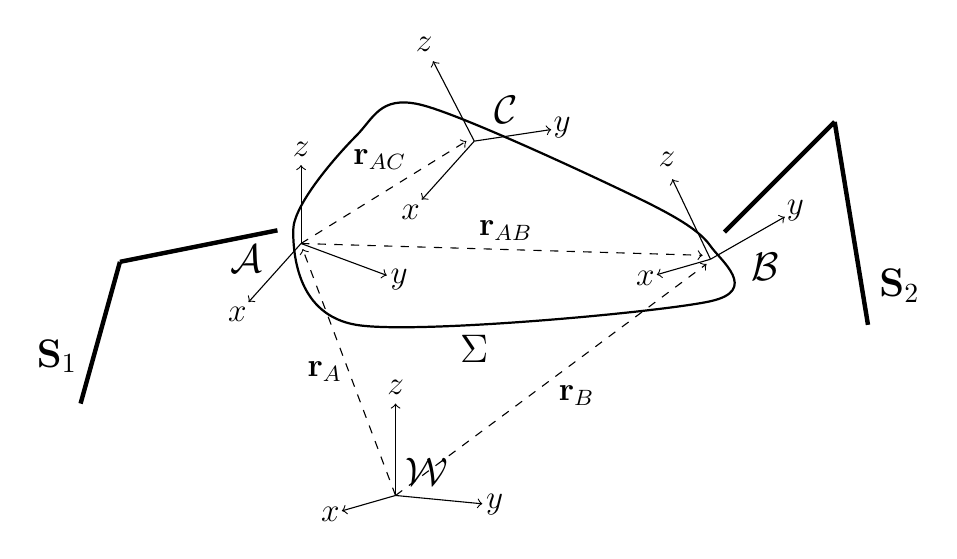
\begin{tikzpicture}[
        media/.style={font={\footnotesize\sffamily}},
        interface/.style={
            % The border decoration is a path replacing decorator.
            % For the interface style we want to draw the original path.
            % The postaction option is therefore used to ensure that the
            % border decoration is drawn *after* the original path.
            postaction={draw,decorate,decoration={border,angle=-45,
            amplitude=0.3cm,segment length=2mm}}},
        ]
        % Object
        \draw [black, thick] plot [smooth cycle] coordinates {
            (2.7, 2.2) (3.5, 3.4) (4.3, 3.8) 
            (7.1, 2.6) (8.0, 2.0) (8.0, 1.3) 
            (3.5, 1.0)
        };
        \draw[media] (5.0, 0.7) node {\Large $\boldsymbol \Sigma$};

        % p_A
        \draw[black, ->, dashed](4.000, -1.167) -- (2.800 + 0.02, 2.033 - 0.07);
        \draw[media] (3.1, 0.40) node {\large $\mathbf{r}_A$}; 
        % p_B
        \draw[black, ->, dashed](4.000, -1.167) -- (8.000 - 0.05, 1.833 - 0.06);
        \draw[media] (6.3, 0.1) node {\large $\mathbf{r}_B$}; 
        % p_AB
        \draw[black, ->, dashed](2.800, 2.033) -- (8.000 - 0.1, 1.833 + 0.05);
        \draw[media] (5.4, 2.2) node {\large $\mathbf{r}_{AB}$};
        % p_AC
        \draw[black, ->, dashed](2.800, 2.033) -- (5.000 - 0.1,  3.333);
        \draw[media] (3.8, 3.1) node {\large $\mathbf{r}_{AC}$};

        % world frame
        \draw[black, ->](4.000, -1.167) -- (5.102, -1.273);
        \draw[black, ->](4.000, -1.167) -- (4.000, 0.000);
        \draw[black, ->](4.000, -1.167) -- (3.318, -1.363);
        \drawdot{4.000}{-1.167}
        \draw[media] (4.400, -0.867) node {\Large $\mathcal{W}$}; 
        \draw[media] (5.260, -1.288) node {\large $y$}; 
        \draw[media] (4.000, 0.200) node {\large $z$}; 
        \draw[media] (3.172, -1.406) node {\large $x$}; 

        % A frame
        \draw[black, ->](2.800, 2.033) -- (3.889, 1.628);
        \draw[black, ->](2.800, 2.033) -- (2.800, 3.029);
        \draw[black, ->](2.800, 2.033) -- (2.133, 1.289);
        \drawdot{2.800}{2.033}
        \draw[media] (2.100, 1.833) node {\Large $\mathcal{A}$}; 
        \draw[media] (4.045, 1.570) node {\large $y$}; 
        \draw[media] (2.800, 3.230) node {\large $z$}; 
        \draw[media] (1.990, 1.130) node {\large $x$}; 

        % B frame
        \draw[black, ->](8.000, 1.833) -- (8.943, 2.371);
        \draw[black, ->](8.000, 1.833) -- (7.515, 2.850);
        \draw[black, ->](8.000, 1.833) -- (7.318, 1.637);
        \drawdot{8.000}{1.833}
        \draw[media] (8.700, 1.733) node {\Large $\mathcal{B}$};
        \draw[media] (9.078, 2.448) node {\large $y$};
        \draw[media] (7.446, 3.100) node {\large $z$};
        \draw[media] (7.172, 1.594) node {\large $x$};

        % C frame
        \draw[black, ->](5.000, 3.333) -- (5.977, 3.480);
        \draw[black, ->](5.000, 3.333) -- (4.476, 4.349);
        \draw[black, ->](5.000, 3.333) -- (4.333, 2.589);
        \drawdot{5.000}{3.333}
        \draw[media] (5.400, 3.733) node {\Large $\mathcal{C}$}; 
        \draw[media] (6.116, 3.501) node {\large $y$}; 
        \draw[media] (4.364, 4.566) node {\large $z$}; 
        \draw[media] (4.190, 2.430) node {\large $x$}; 

        % Draw first manipulator
        \draw[black, ultra thick](0, 0) -- (0.5, 1.8);
        \draw[black, ultra thick](0.5, 1.8) -- (2.5, 2.2);
        % Gripper
        \gripper{2.5}{2.2}{3.3}{2.36}
        % Draw second point mass
        \drawpointmasssimple{0.5}{1.8}
        \base{0}{0}
        \draw[media] (-0.3, 0.6) node {\Large $\mathbf{S}_1$};
        
        % % Draw the second manipulator
        \draw[black, ultra thick](10, 1) -- (9.577, 3.577);
        \draw[black, ultra thick](9.577, 3.577) -- (8.177, 2.177);
        % % Gripper
        \gripper{8.177}{2.177}{7.6}{1.6}
        % % Draw second point mass
        \drawpointmasssimple{9.577}{3.577}
        \base{10}{1}
        \draw[media] (10 + 0.4, 1 + 0.5) node {\Large $\mathbf{S}_2$};
    \end{tikzpicture}
    \caption{Rigid body ($\boldsymbol{\Sigma}$) coupling with fixed frame on it}
    \label{fig:rigid_body_with_fixed_frame}
\end{figure}

It is easy to see that control law in this case is similar to equation 
(\ref{eqn:kinematic_dif_eqn_simple}). The key difference is that target frame has 
no Jacobians to represent frame velocities. Also it is necessary to add acceleration 
part to $\mathbf{b}$. It leads to 

\begin{equation}
    \begin{aligned}
        A & =
        \begin{bmatrix}
            \tilde{J}_v \\
            \tilde{J}_{\omega}
        \end{bmatrix} \\
        \mathbf{b} & = 
        -\begin{bmatrix}
            \dot{\tilde{J}}_v \\
            \dot{\tilde{J}}_{\omega}
        \end{bmatrix}
        \mathbf{v}
        - \begin{bmatrix}
          \mathbf{a}_D \\
          \boldsymbol{\epsilon}_D^{\mathcal{D}}  
        \end{bmatrix}
        - K_d
        \begin{bmatrix}
            \boldsymbol{\upsilon}_d \\
            \boldsymbol{\omega}_d^{\mathcal{D}}
        \end{bmatrix}
        - K_p
        \mathbf{e}_{\SE}(
            T_{\mathcal{W}}^{\mathcal{E}} \cdot
            T_{\mathcal{A}}^{\mathcal{C}}, 
            T_{\mathcal{W}}^{\mathcal{D}}
        )
    \end{aligned}
    \label{eqn:a_and_b_control_rigid_b}
\end{equation}

where $\boldsymbol{\upsilon}_d$, $\boldsymbol{\omega}_d^{\mathcal{D}}$, 
$\tilde{J}_v$, $\tilde{J}_{\omega}$, $\dot{\tilde{J}}_v$, and 
$\dot{\tilde{J}}_{\omega}$ are

\begin{equation}
    \begin{aligned}
        \boldsymbol{\upsilon}_d & = \boldsymbol{\upsilon}_D - 
        \boldsymbol{\upsilon}_E - \boldsymbol{\omega}_E \times \mathbf{r}_{AC} \\
        \boldsymbol{\omega}_d^{\mathcal{D}} & = 
        \boldsymbol{\omega}_D^{\mathcal{D}} - 
        \boldsymbol{\omega}_E^{\mathcal{D}}\\
        \tilde{J}_v & = -J_{E,v} + [R_E \mathbf{r}_{AC}^{\mathcal{A}}]^{\wedge}
        J_{E, \omega} \\
        \tilde{J}_{\omega} & = - R_E^T J_{E, \omega} \\
        \dot{\tilde{J}}_v & = -\dot{J}_{E, v} + 
        \hat{\boldsymbol{\omega}}_E \hat{\mathbf{r}}_{AC} J_{E, \omega} + 
        \hat{\mathbf{r}}_{AC} \dot{J}_{E, \omega} \\
        \dot{\tilde{J}}_{\omega} & = - R_E^T [
            \dot{J}_{E, \omega} - \hat{\boldsymbol{\omega}}_E J_{E, \omega}
        ] 
    \end{aligned}
    \label{eqn:jacobians_for_rigid_control}
\end{equation}

The algorithm is following 

\begin{algorithm}
    \caption{Computing $A$ and $\mathbf{b}$ for control of the connecting 
    rigid body}

    \begin{algorithmic}[1]
        \Function{getRigidBodyControlConstraint}{
            combined system $\mathbf{S}_c$,
            $\mathbf{q}$, $\mathbf{v}$, 
            $E$, $T_{\mathcal{A}}^{\mathcal{C}}$, 
            $T_{\mathcal{W}}^{\mathcal{D}}$, 
            $\begin{bmatrix} \boldsymbol{\upsilon}_D^T & 
            [\boldsymbol{\omega}_D^{\mathcal{D}}]^T \end{bmatrix}^T$, 
            $\begin{bmatrix} \mathbf{a}_D^T & 
            [\boldsymbol{\epsilon}_D^{\mathcal{D}}]^T \end{bmatrix}^T$
        } : 
        \State Compute attitudes $T_{\mathcal{W}}^{\mathcal{E}}$ and 
        velocities $\boldsymbol{\upsilon}_E$, $\boldsymbol{\omega}_E$ 
        for $\mathbf{S}_c$ at state $\mathbf{q}$, $\mathbf{v}$
        \State Obtain Jacobians $J_{E,v}$, $J_{E, \omega}$ and 
        Jacobians time derivatives $\dot{J}_{E,v}$, $\dot{J}_{E, \omega}$ 
        for $\mathbf{S}_c$ at state $\mathbf{q}$, $\mathbf{v}$
        \State Get $\boldsymbol{\upsilon}_d$, $\boldsymbol{\omega}_d^{\mathcal{D}}$, 
        $\tilde{J}_v$, $\tilde{J}_{\omega}$, $\dot{\tilde{J}}_v$, and 
        $\dot{\tilde{J}}_{\omega}$ by equation 
        (\ref{eqn:jacobians_for_rigid_control})
        \State Calculate $A$ and $\mathbf{b}$ by equation 
        (\ref{eqn:a_and_b_control_rigid_b})
        \State \Return $A$, $\mathbf{b}$
        \EndFunction
    \end{algorithmic}
    \label{alg:get_a_and_b_control_rigid}
\end{algorithm}


\section{Task prioritization}
\label{sec:task_prioritization}

After defining algorithm for obtaining $A$ and $\mathbf{b}$ it is necessary to 
consider the prioritization problem. Let's consider the following case. The 
combined system $\mathbf{S}_c$ has $n_v$ degree of freedom. There are $n_c$ 
rigid body constraints and $n_u$ controls laws imposed on it. Thus, the minimal 
requirement for problem to be solvable is

\begin{equation}
    n_v \geq 6 \cdot (n_c + n_u)
\end{equation}

Although this equation is useful for brief estimation, but it is still necessary 
condition. The control issues can arise due to the complex topological structure 
of joint space manifold. Hence, there are two options prove that desired 
trajectory is out off null space, or introduce some prioritization technique.

In the first case, it is enough to use combined matrices: \\
$A = \begin{bmatrix} A_c^T & A_u^T \end{bmatrix}^T$, and 
$\mathbf{b} = \begin{bmatrix} \mathbf{b}_c^T & \mathbf{b}_u^T \end{bmatrix}^T$ 
with the Udwadia-Kalaba approach, where $A_c$, $A_u$, $\mathbf{b}_c$, and 
$\mathbf{b}_u$ are 

\begin{equation}
    \begin{aligned}
        A_c & = \begin{bmatrix}
            A_{c_1}^T & A_{c_2}^T & \dots & A_{c_{n_c}}^T
        \end{bmatrix}^T \\
        A_u & = \begin{bmatrix}
            A_{u_1}^T & A_{u_2}^T & \dots & A_{u_{n_u}}^T
        \end{bmatrix}^T \\
        \mathbf{b}_c &= \begin{bmatrix}
            \mathbf{b}_{c_1}^T & \mathbf{b}_{c_2}^T & \dots & 
            \mathbf{b}_{c_{n_c}}^T
        \end{bmatrix}^T \\
        \mathbf{b}_u &= \begin{bmatrix}
            \mathbf{b}_{u_1}^T & \mathbf{b}_{u_2}^T & \dots & 
            \mathbf{b}_{u_{n_u}}^T
        \end{bmatrix}^T \\
    \end{aligned}
    \label{eqn:combined_a_and_b}
\end{equation}

However, the discussed approach is not general. It is rare to proof 
controllability in real life cases. 

The second way to figure out the problem is prioritization. The most rigorous 
technique to achieve is utilizing null space. Generally, it is preferable to 
strongly preserve the rigid body constraints and try to find the least square 
solution for control task. Such method can be expressed as 

\begin{equation}
    \begin{aligned}
        \min_{\dot{\mathbf{v}}} \quad & 
        [A_u \dot{\mathbf{v}} - \mathbf{b}_u]^T 
        [A_u \dot{\mathbf{v}} - \mathbf{b}_u]\\
        \textrm{s.t.} \quad & \dot{\mathbf{v}} = A_c^{+} \mathbf{b}_c + 
        \dot{\mathbf{v}}_u \\ 
        \quad & \dot{\mathbf{v}}_u \in \mathcal{N}(A_c)
    \end{aligned}
    \label{eqn:task_prior_null_space}
\end{equation}

The above optimization prioritization is analytically solvable but solution 
is not convenient to use in terms of equation (\ref{eqn:gauss_least_const}). 
Therefore, it is easy to reformulate the Gauss least constraint principle and 
include prioritization:

\begin{equation}
    \begin{aligned}
        \min_{\dot{\mathbf{v}}} \quad &
        [\dot{\mathbf{v}} - \mathbf{a}]^T M [\dot{\mathbf{v}} - \mathbf{a}] +
        \omega 
        [A_u \dot{\mathbf{v}} - \mathbf{b}_u]^T 
        [A_u \dot{\mathbf{v}} - \mathbf{b}_u]\\
        \textrm{s.t.} \quad &
        A_c \dot{\mathbf{v}} = \mathbf{b}_c \\
        &
        \mathbf{a} = M^{-1} \mathbf{Q}
    \end{aligned}
    \label{eqn:gauss_least_const_prior}
\end{equation}

where $\omega > 0$ tunable parameter. Due to $M \succcurlyeq 0 $ and 
$A_u^T A_u \succcurlyeq 0$ the optimization problem 
(\ref{eqn:gauss_least_const_prior}) is quadratic task. Hence, it is always
has a solution and can be solved fast by modern frameworks.
